\section*{Appendix}
\label{Appendix Section}

\begin{table}[H]
    \begin{center}
     \footnotesize
     \begin{tabular}{|c||c|c|c|c|c|c|c|c|c|c|}
     \hline
     \multicolumn{11}{|c|}{Score of 10-fold cross-validation} \\
     \hline \hline
     n-fold & 1 & 2 & 3 & 4 & 5 & 6 & 7 & 8 & 9 & 10 \\
     \hline
     Score & 0.911& 0.933 &0.911 &0.911 &0.8 & 0.911&0.864 &0.9318 &0.8182 &0.8182 \\
     \hline
     \end{tabular} \\ 
     \caption{Tabular results of the score of 10-fold cross-validation}
     \label{10fold score}
    \end{center}
\end{table}

    \begin{table}[H]
        \begin{center}
         \footnotesize
         \begin{tabular}{|c||c|}
         \hline
         Accuracy Score& 0.9080717488789237 \\
         \hline
         Test Score & 0.9080717488789237\\
         \hline
         Train Score& 0.988450433108758\\
         \hline
         Test Error& 0.09192825112107628\\
         \hline
         Train Error&0.011549566891241536\\
         \hline
         \end{tabular} \\ 
         \caption{Tabular results of the overall scores of the algorithm}
         \label{scores}
        \end{center}
    \end{table}

\begin{figure}[H]
\centering
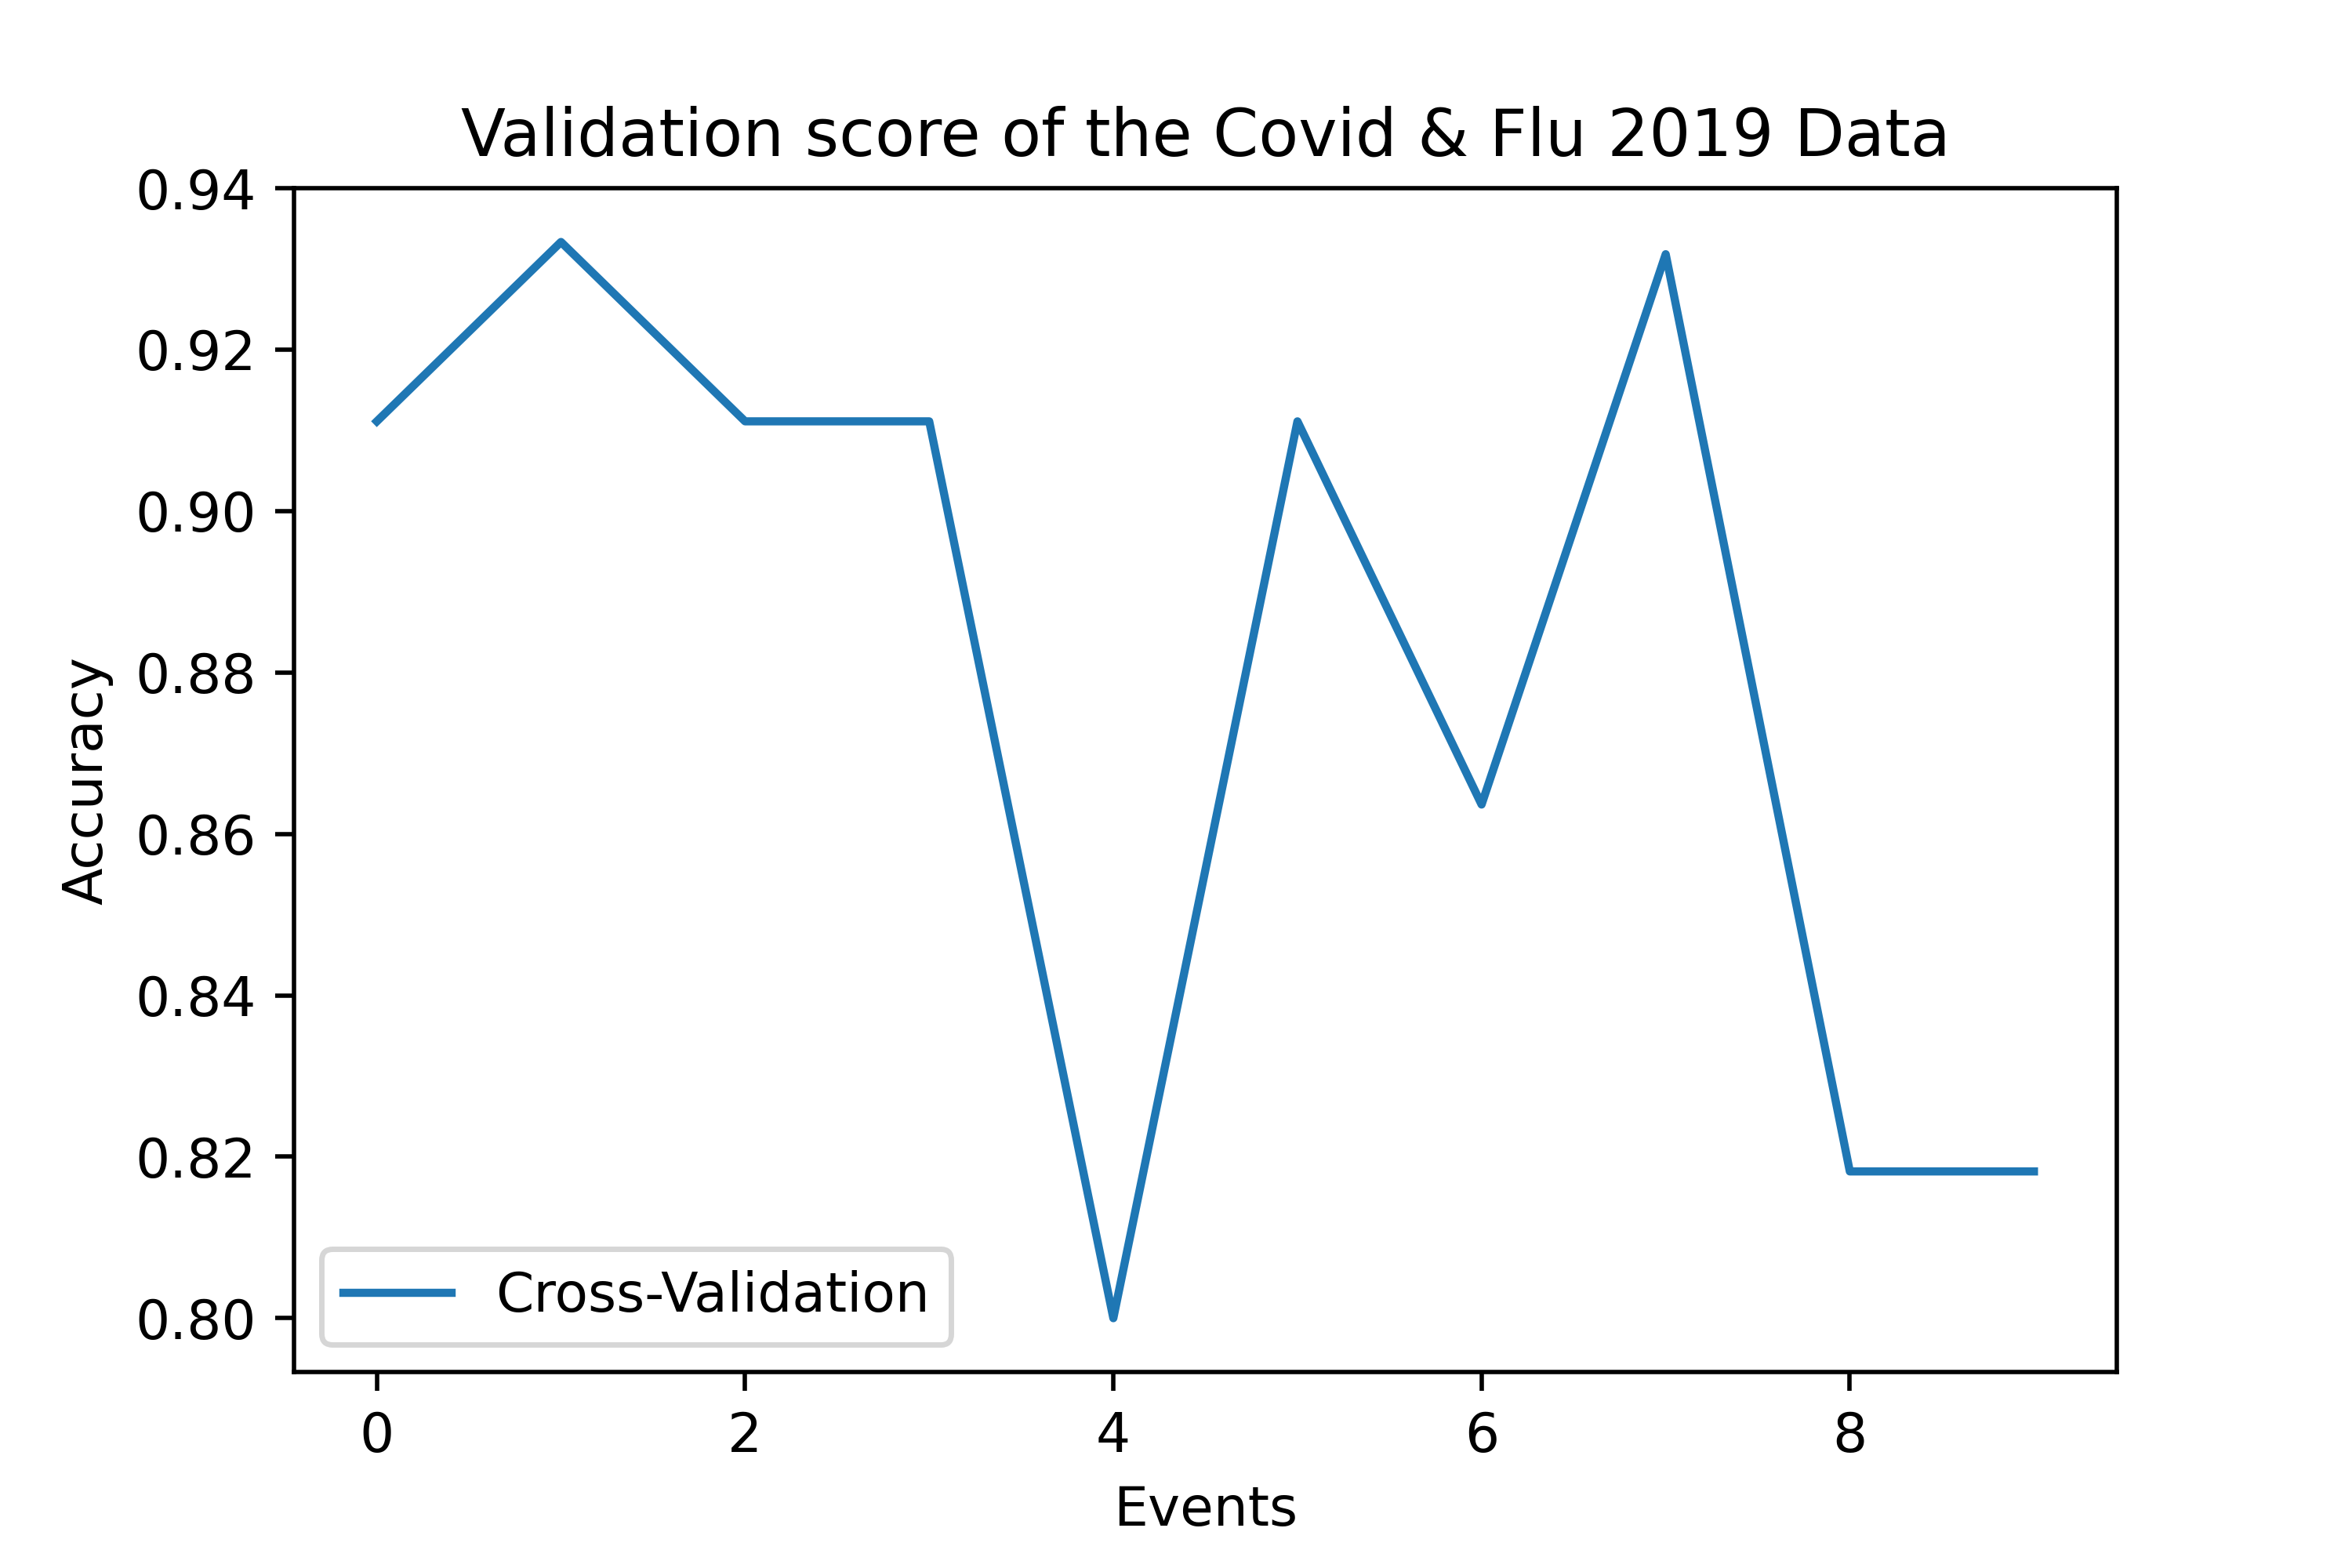
\includegraphics[scale=1]{Media/MediaContent/ScoreValidation.png}
\caption{A figure displaying the score validation of the training algorithm using samples from the Covid and Flu 2019 data census.}
\label{ValScore}
\end{figure}

\begin{figure}[H]
\centering
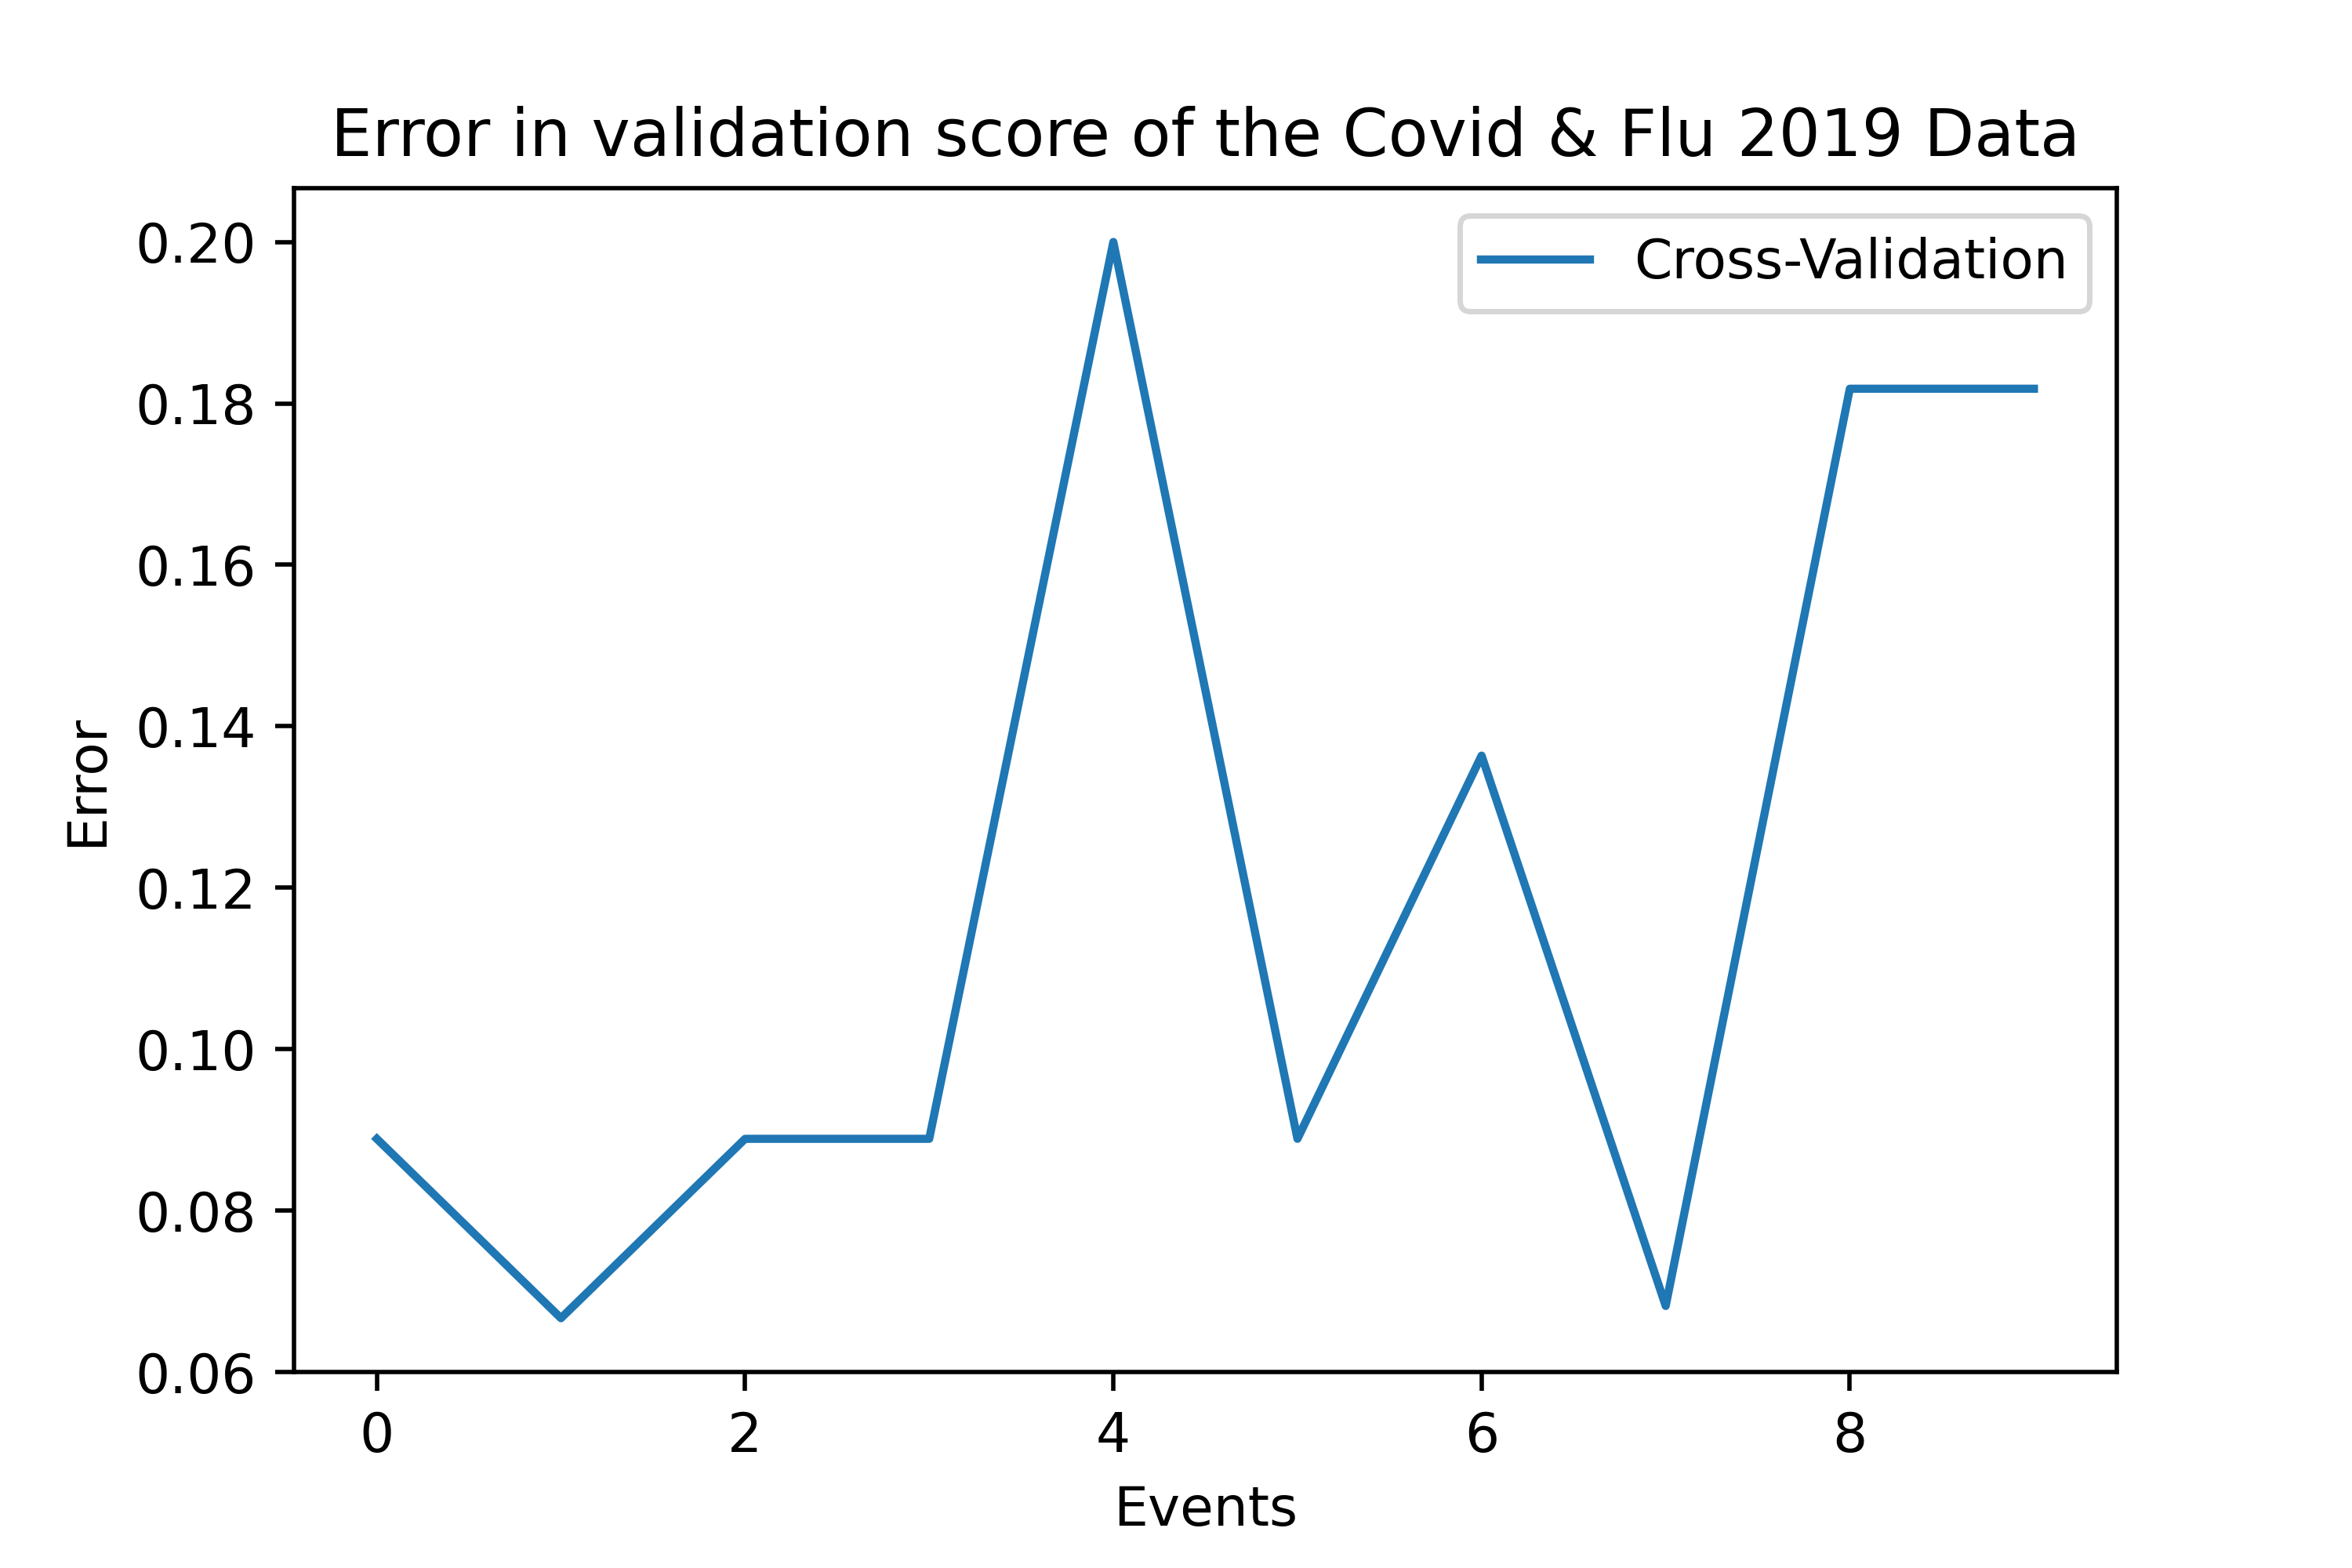
\includegraphics[scale=1]{Media/MediaContent/ErrorInValidation.png}
\caption{A figure displaying the error in the score validation of the training algorithm using samples from the Covid and Flu 2019 data census.}
\label{ErrScore}
\end{figure}

\newpage
\begin{figure}[H]
\centering
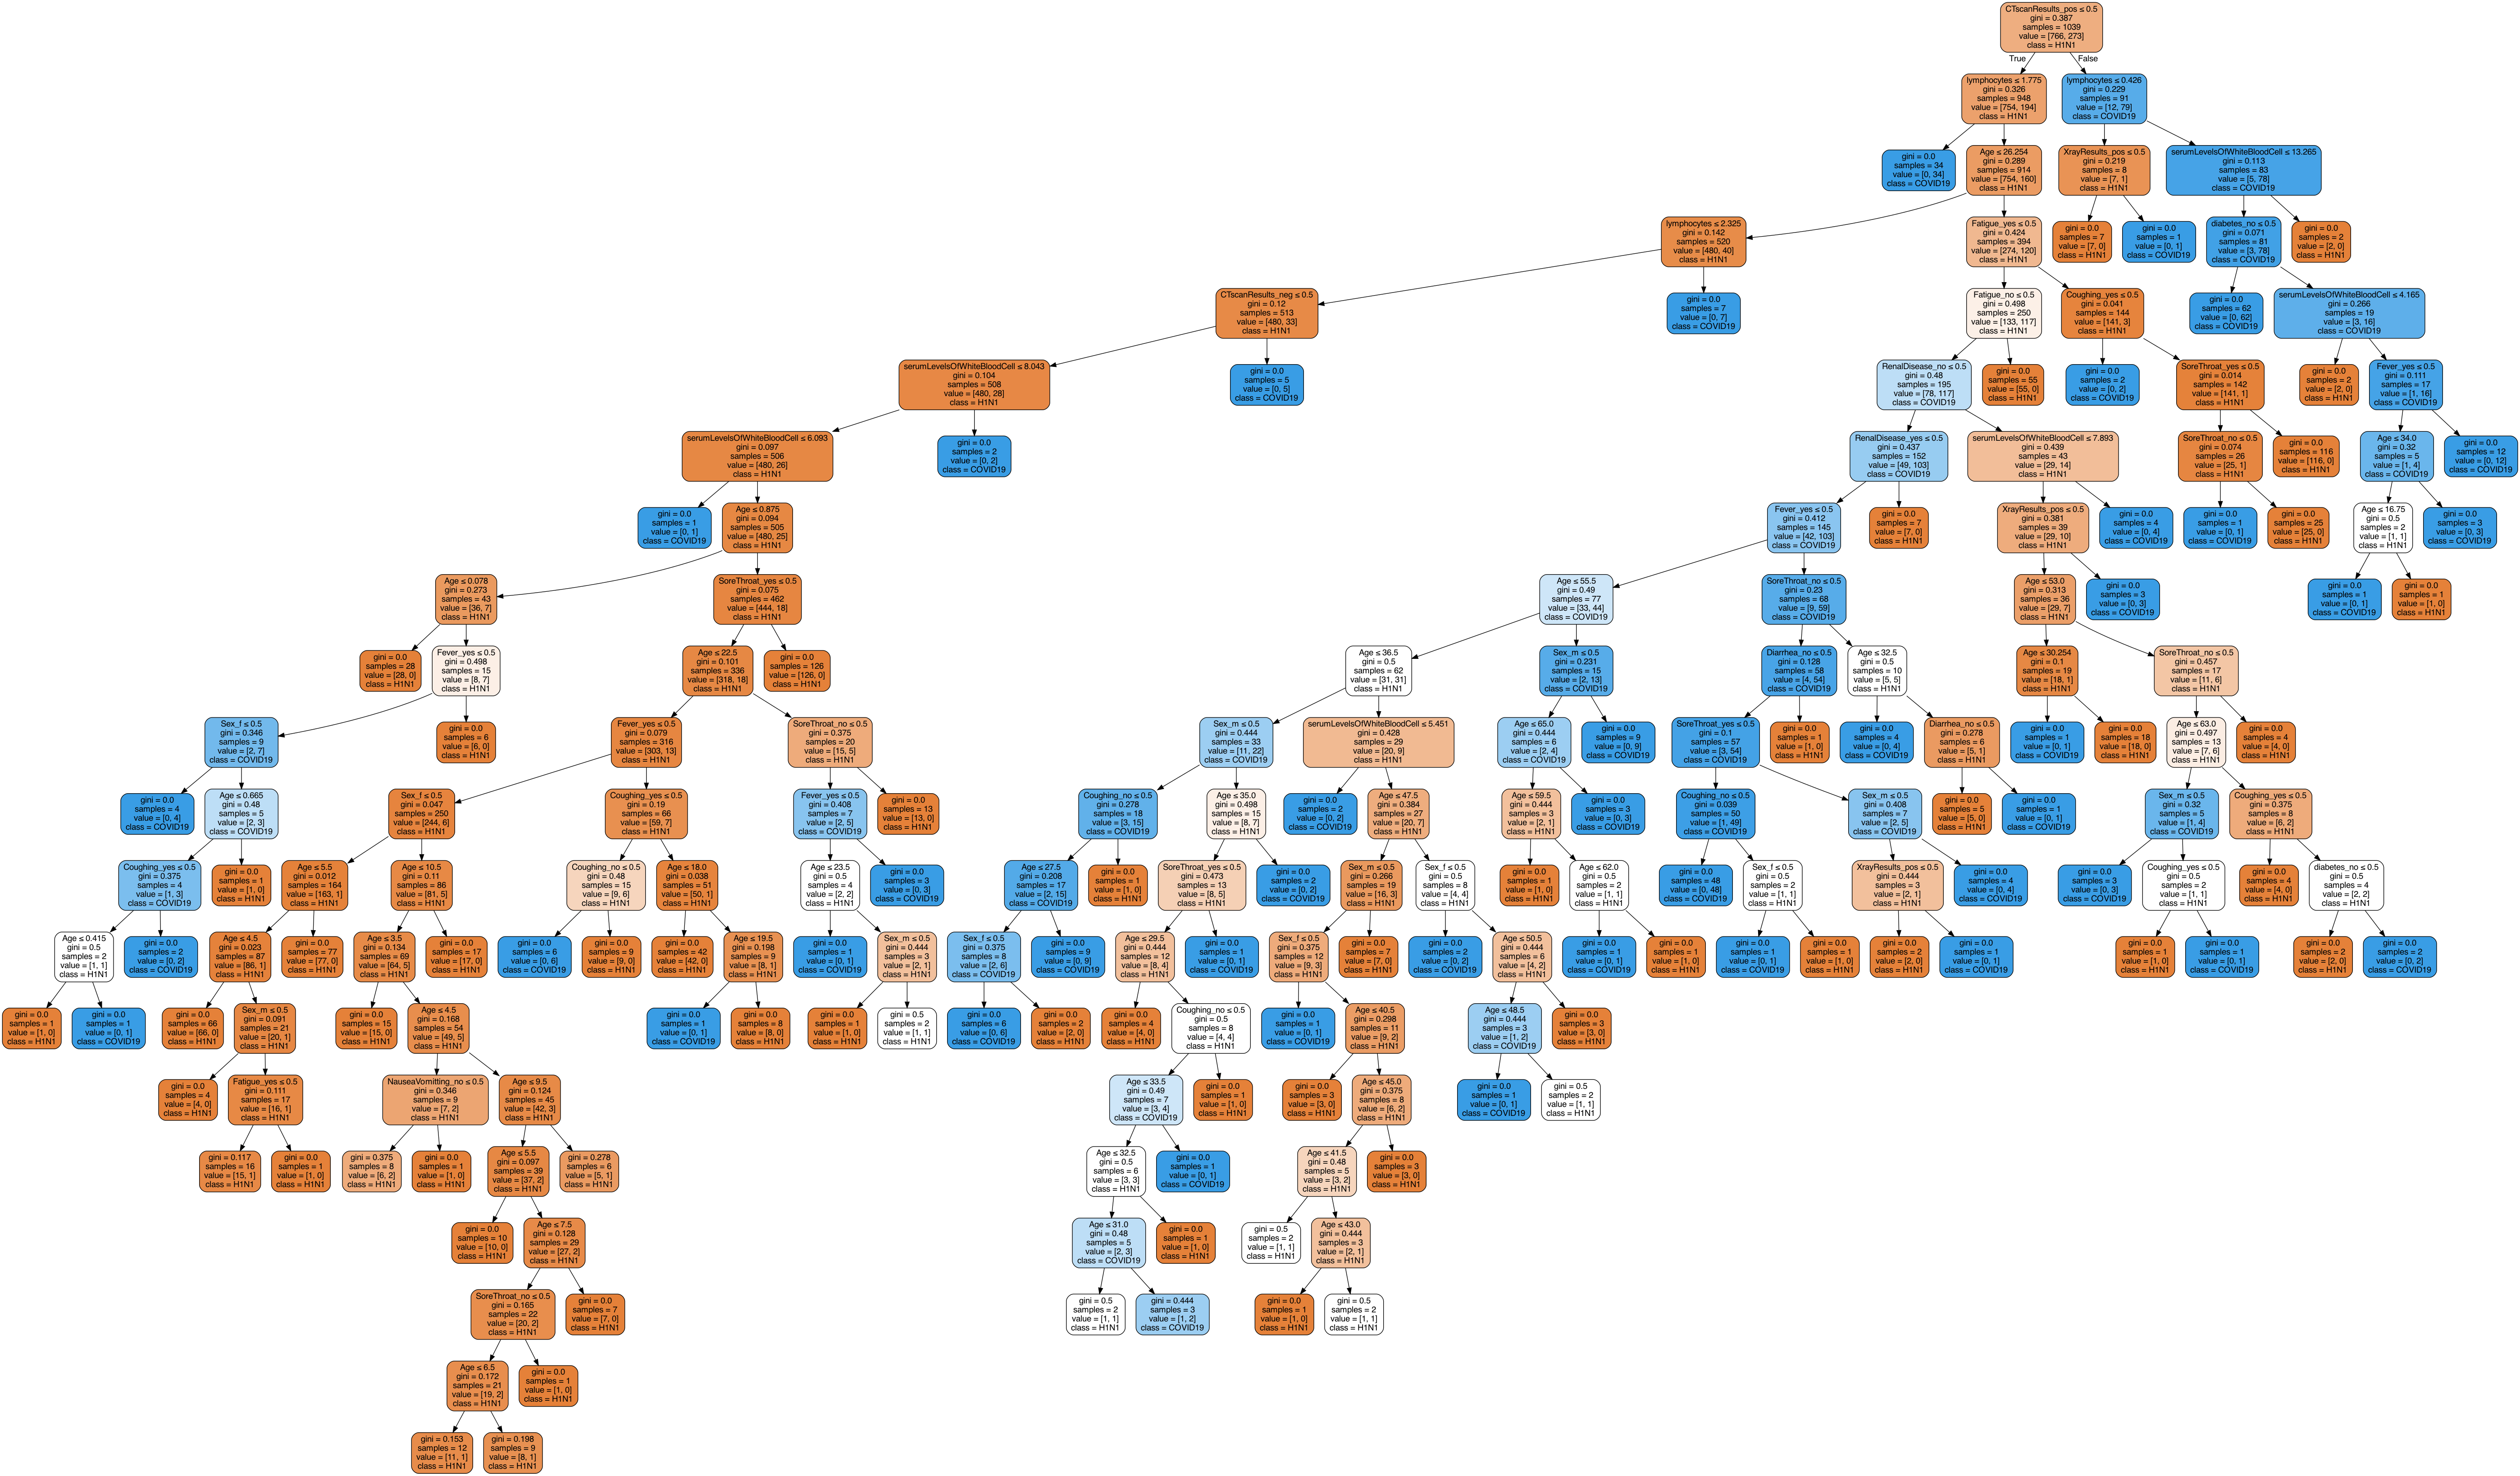
\includegraphics[angle=90, origin=c, scale=0.12]{Media/MediaContent/DecisionTree.png}
\caption{A generated decision tree based off of the algorithm using samples from the Covid and Flu 2019 data census.}
\label{DecTree}
\end{figure}